\documentclass[12pt, letterpaper]{article}
\usepackage[utf8]{inputenc}
\usepackage{amsmath}
\usepackage{amsthm}
\usepackage{amssymb}
\usepackage{colortbl}
\usepackage{xcolor}
\usepackage{fancyvrb}
\usepackage{listings}
\definecolor{anti-flashwhite}{rgb}{0.95, 0.95, 0.96}
\lstset{
    backgroundcolor=\color{anti-flashwhite},
    basicstyle=\ttfamily\footnotesize,
    breakatwhitespace=false,         
    breaklines=true,                 
    captionpos=b,                    
    keepspaces=true,                 
    numbers=left,                    
    numbersep=5pt,                  
    showspaces=false,                
    showstringspaces=false,
    showtabs=false,                  
    tabsize=2
}

\usepackage[a4paper, total={6.5in, 10in}]{geometry}
\usepackage{graphicx}
\graphicspath{ {/} }
\newtheorem{problem}{Problema}
\title{Computación Concurrente - Tarea 4}
\author{Damián Rivera González\\Alexis Hernandez Castro}

\begin{document}
\maketitle

\begin{itemize}
\item[1.] Para cada una de las siguientes ejecuciones contesta lo siguiente: \\
$\textbf{Inciso a)}$
\begin{itemize}
\item ¿Qué es $H|B$?\\
$<B, cp.deq(b)>\\
<B, cp.dep(c)>$
\item ¿Qué es $H|r$?
No existe el objeto r
\item Transforma H en una subhistoria H'\\
$<A, cp.enq(a,3)>\\
<B, cp.deq(b)>\\
<A, cp:void>\\
<A, cp.enq(b,2)>\\
<A, cp:void>\\
<B, cp:b>\\
<B, cp.deq(c)>\\
<B, cp:c>$
\item ¿H' está bien formada?
Sí, porque la proyección del hilo A y B son secuenciales
\item ¿H' secuencial?
No, porque las invocaciones de métodos no tienen inmediatamente su regreso
\item ¿H' es linearizable? Marca los puntos de linearizabilidad.
No es linearizable, porque se hace la invocación de $<B, cp.deq(c)>$ sin embargo, c no ha sido ingresado en la cola.
\end{itemize}

$\textbf{Inciso b)}$
\begin{itemize}
\item ¿Qué es $H|B$?\\
$
<B, r.write(1)>\\
<B, r:void>\\
<B, r.read(1)>\\
<B, r:1>\\
$
\item ¿Qué es $H|r$?
$
<B, r.write(1)>\\
<A, r.read(1)>\\
<C, r.write(2)>\\
<A, r: 1>\\
<B, r:void>\\
<C, r:void>\\
<B, r.read(1)>\\
<B, r:1>\\
<C, r.read(?)>
$
\item Transforma H en una subhistoria H'
$
<B, r.write(1)>\\
<A, r.read(1)>\\
<C, r.write(2)>\\
<A, r: 1>\\
<B, r:void>\\
<C, r:void>\\
<B, r.read(1)>\\
<B, r:1>\\
<A, q.write(3)>
<A, q:void>
$
\item ¿H' está bien formada?
Sí, porque la proyección de cada hilo es secuencial
\item ¿H' secuencial?
No, porque las invocaciones no tienen inmediatamente su regreso
\item ¿H' es linearizable? Marca los puntos de linearizabilidad.
Si es linearizable.
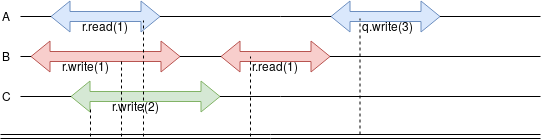
\includegraphics[width=0.9\textwidth]{1b_linearizable.png}\\

\end{itemize}
\item[2. ] Para cada una de las siguientes historias, reconstruye su ejecución y menciona
si cumple con la propiedad de consistencia secuencial, de quietud y/o es
linearizable. Marca los puntos de linearizabilidad.
\begin{itemize}
\item[a)]
$
<C, r.write(1)>\\
<B, r.read>\\
<A, r.write(2)>\\
<B, r: 1>\\
<A, r: void>\\
<C, r: void>\\
<C, r.read>\\
<C, r: 2>
$\\
Sí cumple con la propiedad de consistencia secuencial, de quietud y es linearizable\\
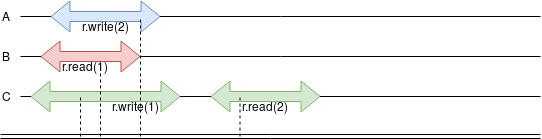
\includegraphics[width=0.9\textwidth]{2a.png}\\
\item[b)]
$
<A, q.enq(1)>\\
<B, q.deq()>\\
<C, q.enq(2)>\\
<B, q: 2>\\
<C, q: void>\\
<A, q: void>\\
<B, q.deq()>\\
<B, q: 1>
$\\
Sí cumple con la propiedad de consistencia secuencial, de quietud y es linearizable\\
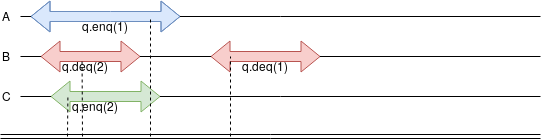
\includegraphics[width=0.9\textwidth]{2b.png}\\
\item[c)]
$
<B, r.write(1)>\\
<A, r.read()>\\
<C, r.write(2)>\\
<A, r: 1>\\
<B, r: void>\\
<C, r: void>\\
<B, r.read()>\\
<B, r: 1>
$\\
Sí cumple con la propiedad de consistencia secuencial, de quietud y es linearizable\\
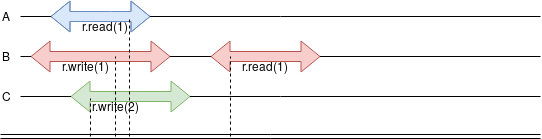
\includegraphics[width=0.9\textwidth]{2c.png}\\
\end{itemize} 

\item[3. ] Para las historias H que hayan sido linearizables tanto en el primer como en el tercer ejercicio, da la historia linearizable. Justitifica que es legal y muestra el conjunto de relaciones de precedencia que deben cumplirse.\\
Para todas las historias es legal porque en cada una se trabaja sobre un mismo objeto (ya sea $r$ o $q$) y la proyección de cada objeto es la misma historia que damos (con excepción de la historia 1a, pero ambas proyecciones de los objetos están en la especificación secuencial de cada objeto) , la cual está en la especificación secuencial del objeto.\\
$\textbf{Historia 1b}\\
<C, r.write(2)>\\
<C, r:void>\\
<B, r.write(1)>\\
<B, r:void>\\
<A, r.read(1)>\\
<A, r:1>\\
<B, r.read(1)>\\
<B, r:1>\\
<A, q.write(3)>\\
<A, q:void>
$\\
Precedencia = $\{r.write(2) \rightarrow r.write(1), r.write(1) \rightarrow r.read(1), r.read(1) \rightarrow q.write(3)\}$ más todas las relaciones de precedencia que se dan por la transitividad

$\textbf{Historia 2a}\\
<C, r.write(1)>\\
<C, r:void>\\
<B, r.read(1)>\\
<B, r:1>\\
<A, r.write(2)>\\
<A, r:void>\\
<C, r.read(2)>\\
<C, r:2>\\
$\\
Precedencia = $\{r.write(1) \rightarrow r.read(1), r.read(1) \rightarrow r.write(2), r.write(2) \rightarrow r.read(2)\}$ más todas las relaciones de precedencia que se dan por la transitividad

$\textbf{Historia 2b}\\
<C, q.enq(2)>\\
<C, q:void>\\
<B, q.deq(2)>\\
<B, q:2>\\
<A, q.enq(1)>\\
<A, q:void>\\
<B, q.deq(1)>\\
<B, q:1>\\
$\\
Precedencia = $\{q.enq(2) \rightarrow q.deq(2), q.deq(2) \rightarrow q.enq(1) \rightarrow q.deq(1) \}$ más todas las relaciones de precedencia que se dan por la transitividad

$\textbf{Historia 3b}\\
<C, r.write(2)>\\
<C, r:void>\\
<B, r.write(1)>\\
<B, r:void>\\
<A, r.read(1)>\\
<A, r:1>\\
<B, r.read(1)>\\
<B, r:1>\\
$\\
Precedencia = $\{ r.write(2) \rightarrow r.write(1), r.write(1) \rightarrow r.read(1), r.read(1) \rightarrow r.read(1)\}$ más todas las relaciones de precedencia que se dan por la transitividad

\item[4. ] Da un ejemplo de una ejecución que tenga consistencia de quietud pero no secuencial; y otra que tenga consistencia secuencial pero no de quietud. Argumenta porque las ejecuciones no cumplen con cada propiedad.\\
$\textbf{Consistencia de quietud, no secuencial}$: No se pueden ordenar las llamadas de los métodos de manera que se lea 1 y 2 sin a ver escrito 2 y 1. Si se leyó 1 debió escribirse 2 y 1, pero ya no se podría leer 2, si se leyó 2 se escribió 2, pero previamente no se pudo haber leído 1.

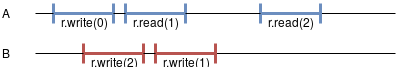
\includegraphics[width=0.9\textwidth]{4_1.png}\\

$\textbf{Consistencia Secuencial, no de quietud}$: Antes del espacio de quietud la última escritura debe ser 0 ó 1, pero después del espacio de quietud se debe poder leer 0 y 1, pero la última escritura solo puede tener un valor. Por lo que si la última escritura (antes del tiempo de quietud) fue 0, no podríamos leer 0 y después 1, y viceversa, si la última escritura (antes del tiempo de quietud) fue 1, no podríamos leer 1 y luego 0.

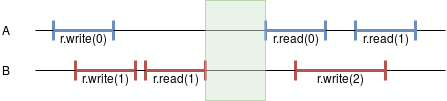
\includegraphics[width=0.9\textwidth]{4_2.png}\\

\item[5. ] Suponiendo que en el sistema existe un solo hilo, ¿Es la consistencia de quietud
equivalente a la consistencia secuencial? Argumenta formalmente.\\
Sí. Veamos la consistencia de quietud de un hilo, llamemosle $A$. Como la ejecución de un hilo es secuencial, entonces cada llamada a un método tiene inmediatamente su regreso
\begin{equation*}
\begin{split}
&...\\
&<A, objeto.metodo()> \\
&<A, objeto:regreso>\\
&...
\end{split}
\end{equation*}  
Con lo cual los tiempos de quietud de la ejecución de un hilo, están entre cada llamada de un método. Por esto si tenemos una llamada $m_i$ que precede a la llamada $m_{i+1}$ esto es $m_i \rightarrow m_{i+1}$ entre cada tiempo de quietud solo podemos reordenar una única llamada a método $m_x$ con lo cual en la consistencia de quietud del hilo A, cada relación de precedencia $m_i \rightarrow m_{i+1}$ se mantiene igual y como la ejecución de un hilo es secuencial entonces la relación de precedencia $m_i \rightarrow m_{i+1}$ en la consistencia secuencial se mantiene igual, por lo que al hacer $H|A$ en la consistencia de quietud será la misma al hacer $H|A$ en la consistencia secuencual.

\item[6 .] Al igual como le hicimos con la linearizabilidad, define formalmente el concepto
de consistencia de quietud. HINT: Define la noción de un bloque sin quietud y agrega la precedencia de eventos $(\rightarrow)$ entre ellos.

\item[7. ]Demuestra por qué la consistencia de $\textbf{quietud}$ es composicional.

\item[8. ] Considera un objeto $p$ que utiliza dos registros. Por el ejercicio anterior, sabemos que si ambos registros cumplen con la consistencia de quietud, entonces $p$ también la cumplirá ¿El caso contrario se cumple? Es decir, si $p$ cumple con la consistencia de quietud entonces los registros también cumplen la consistencia de quietud? Esbozar una prueba o dar un contraejemplo.


\end{itemize}

\end{document}
